\label{Figure Image Rotation}
\begin{figure}[H]
    \centering
    \begin{subfigure}{0.15\textwidth}
        \centering
        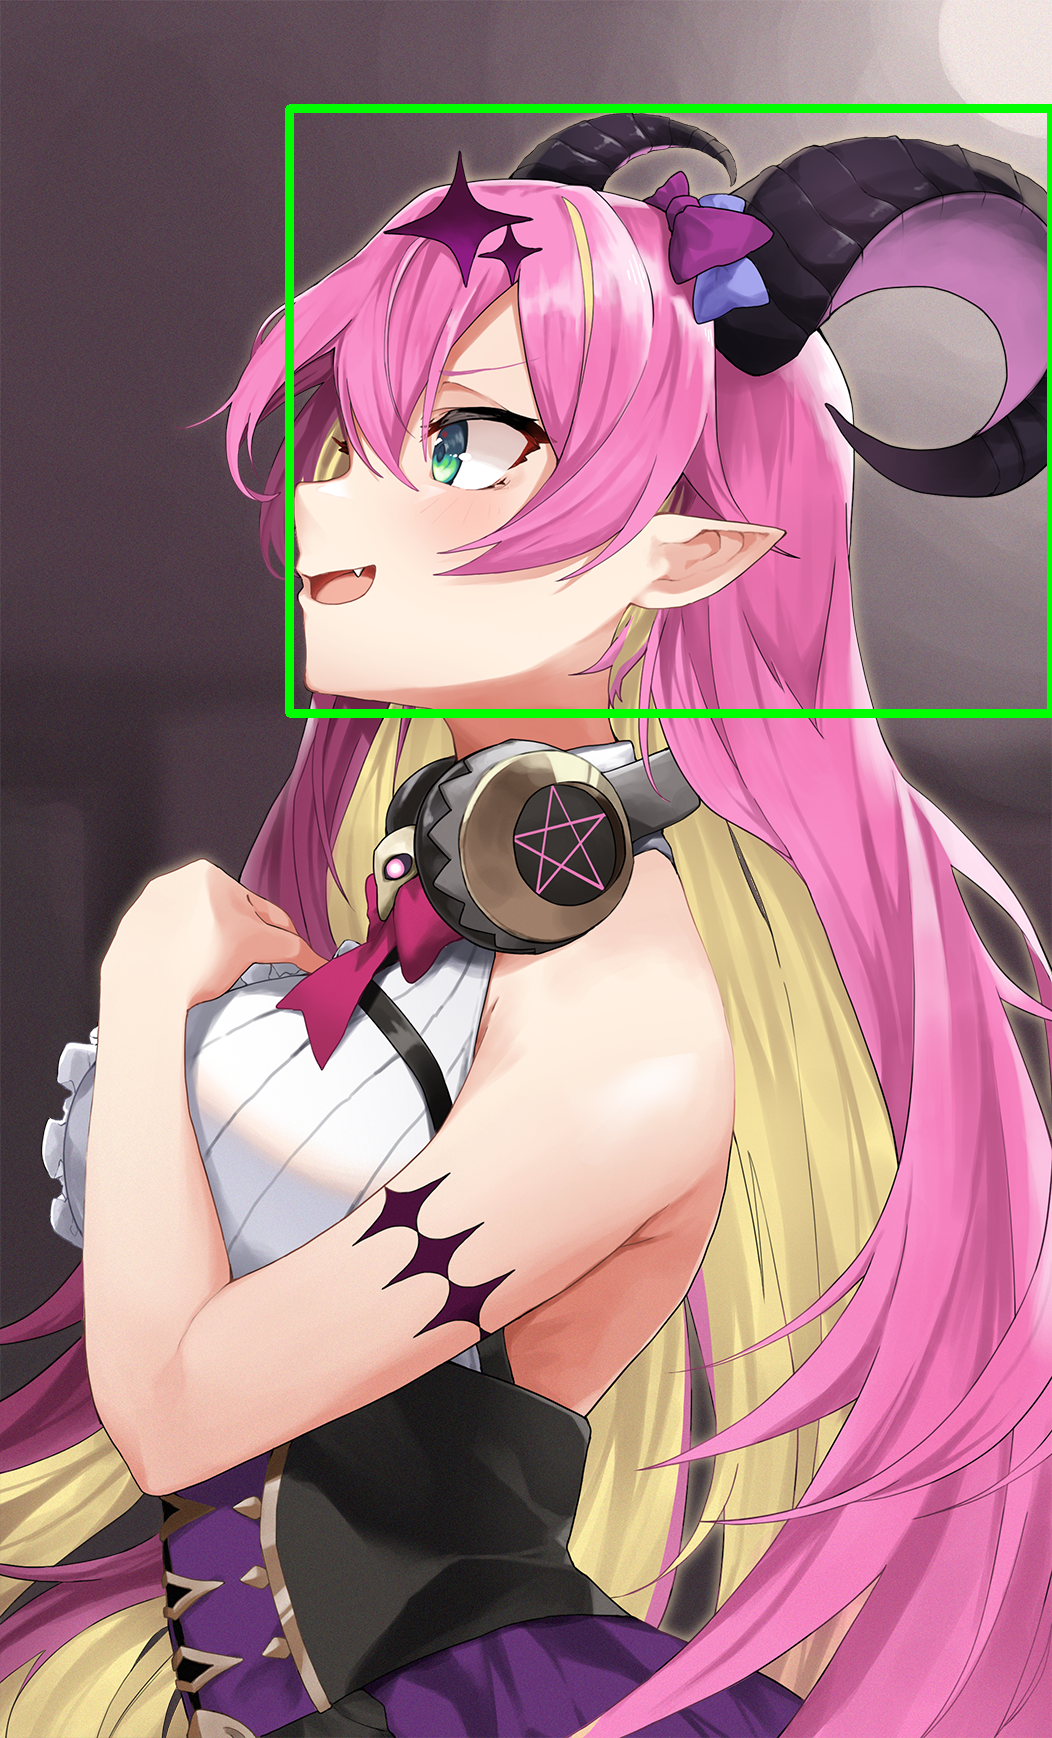
\includegraphics[width=\textwidth]{images/augmentation/Pixiv-83768702_p0-BB.png}
        % \caption{Original}
        \caption{}
        \label{fig:aloe1}
    \end{subfigure}
    \hfill
    \begin{subfigure}{0.15\textwidth}
        \centering
        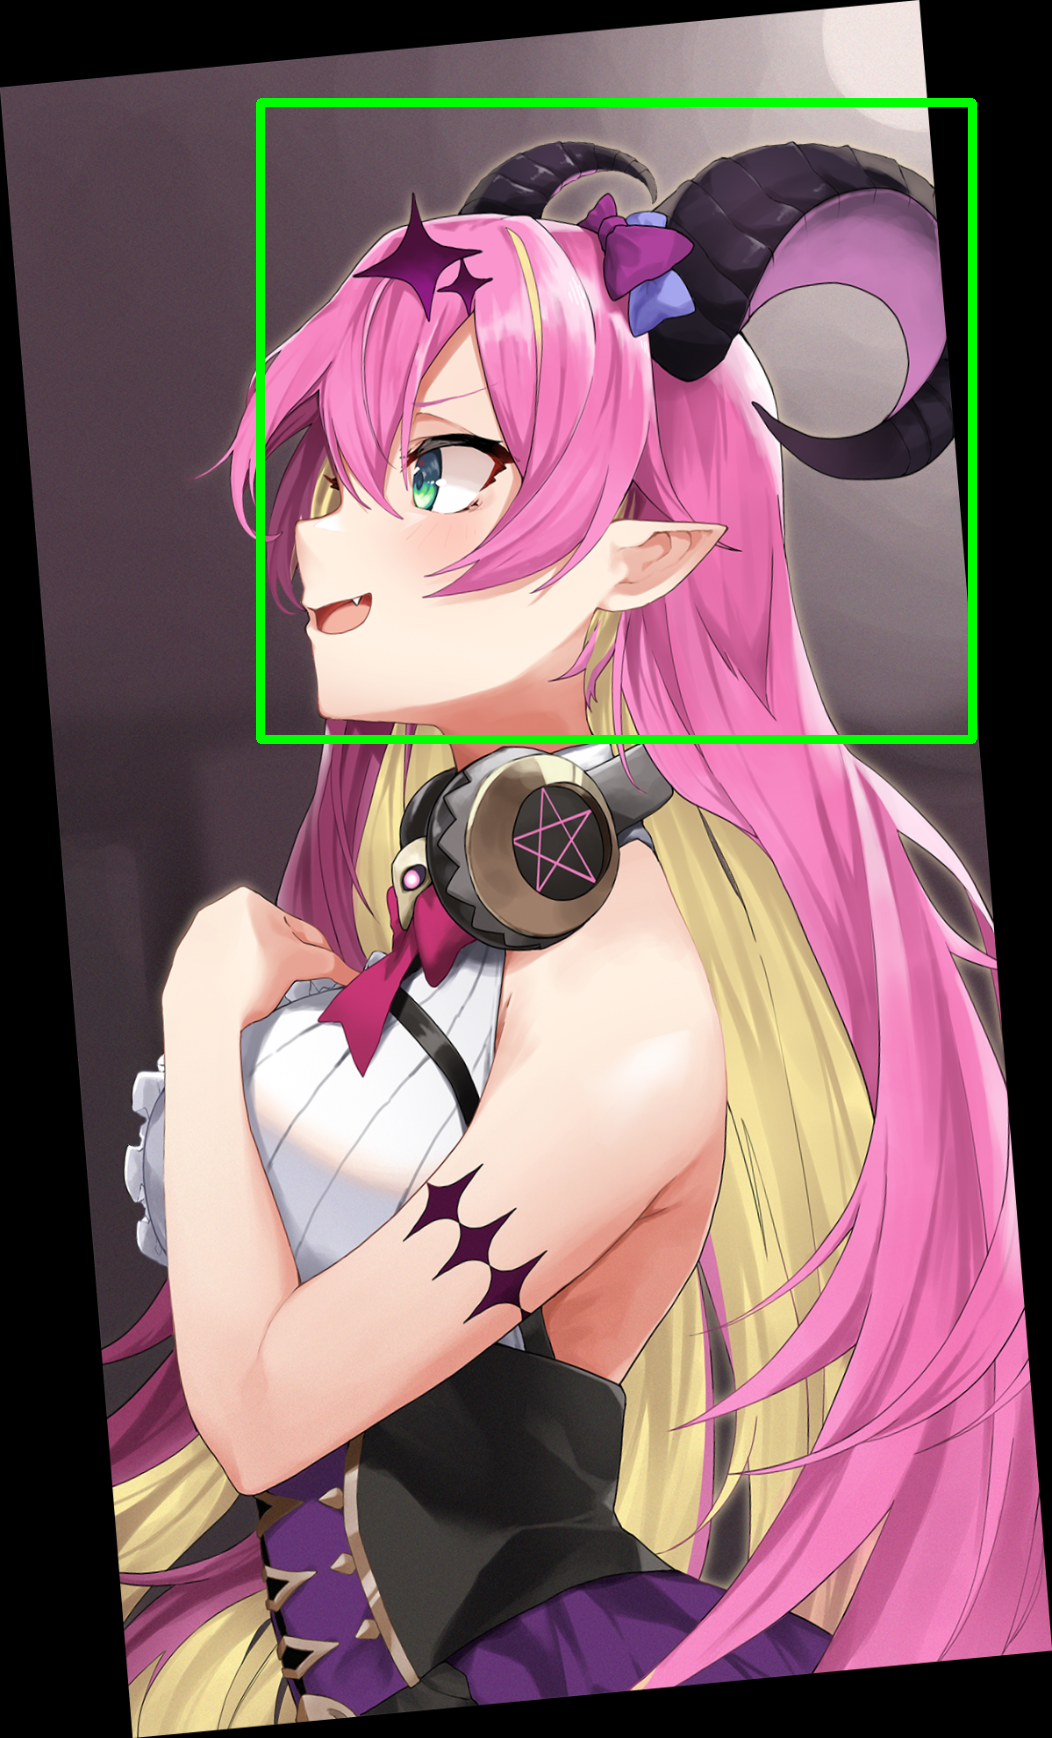
\includegraphics[width=\textwidth]{images/augmentation/Pixiv-83768702_p0-RandomRotate_5-BB.png}
        % \caption{5 degrees}
        \caption{}
        \label{fig:aloe2}
    \end{subfigure}
    \hfill
    \begin{subfigure}{0.15\textwidth}
        \centering
        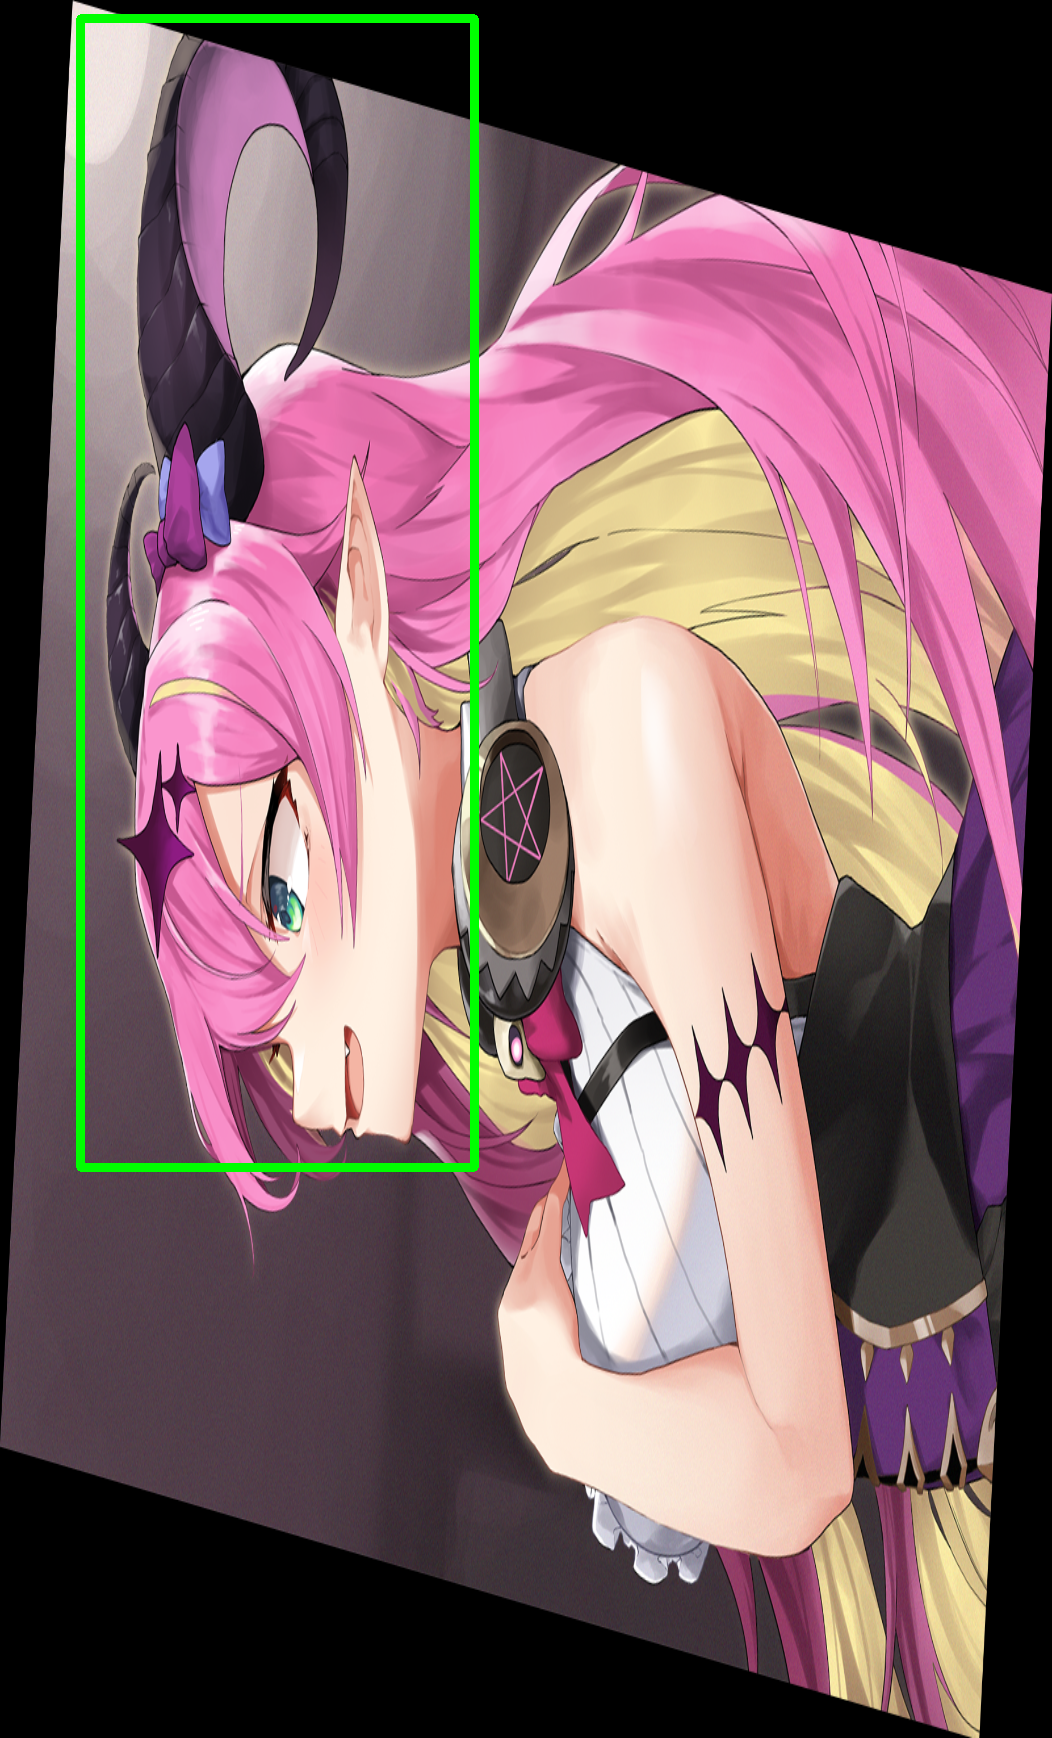
\includegraphics[width=\textwidth]{images/augmentation/Pixiv-83768702_p0-RandomRotate_83-BB.png}
        % \caption{83 degrees}
        \caption{}
        \label{fig:aloe3}
    \end{subfigure}
    \hfill
    \begin{subfigure}{0.15\textwidth}
        \centering
        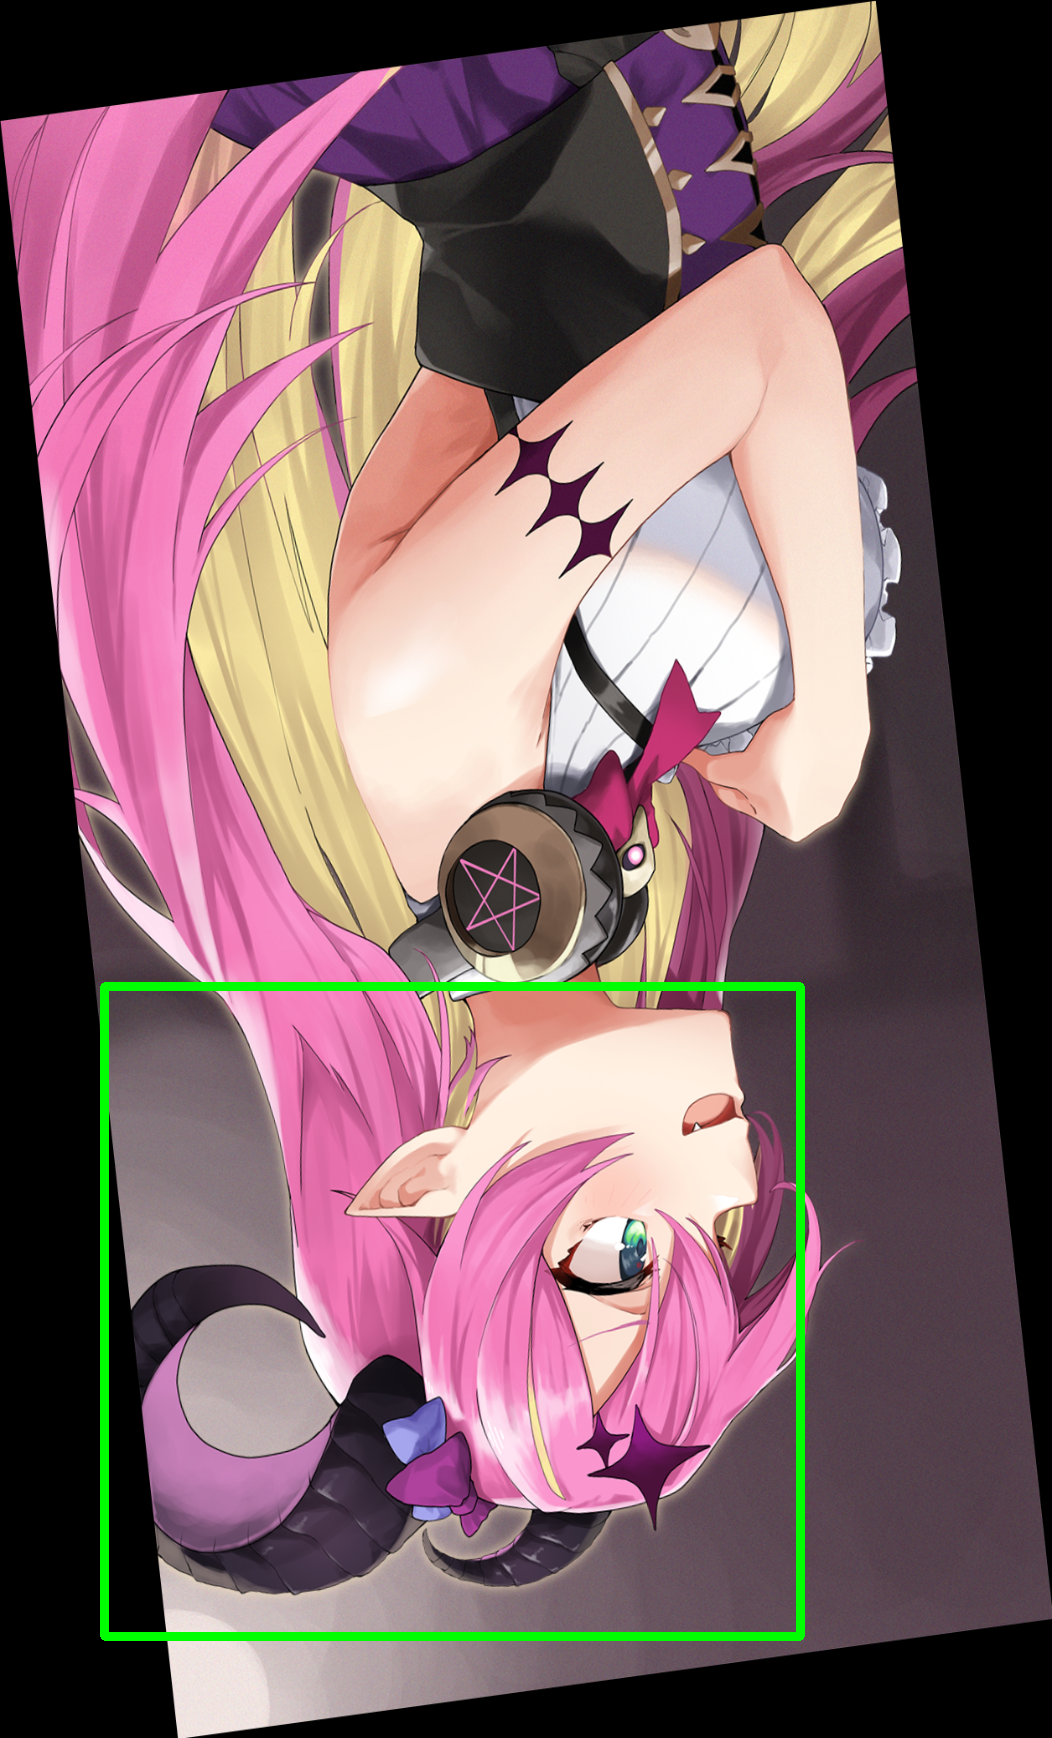
\includegraphics[width=\textwidth]{images/augmentation/Pixiv-83768702_p0-RandomRotate_187-BB.png}
        % \caption{187 degrees}
        \caption{}
        \label{fig:aloe4}
    \end{subfigure}
    \begin{subfigure}{0.15\textwidth}
        \centering
        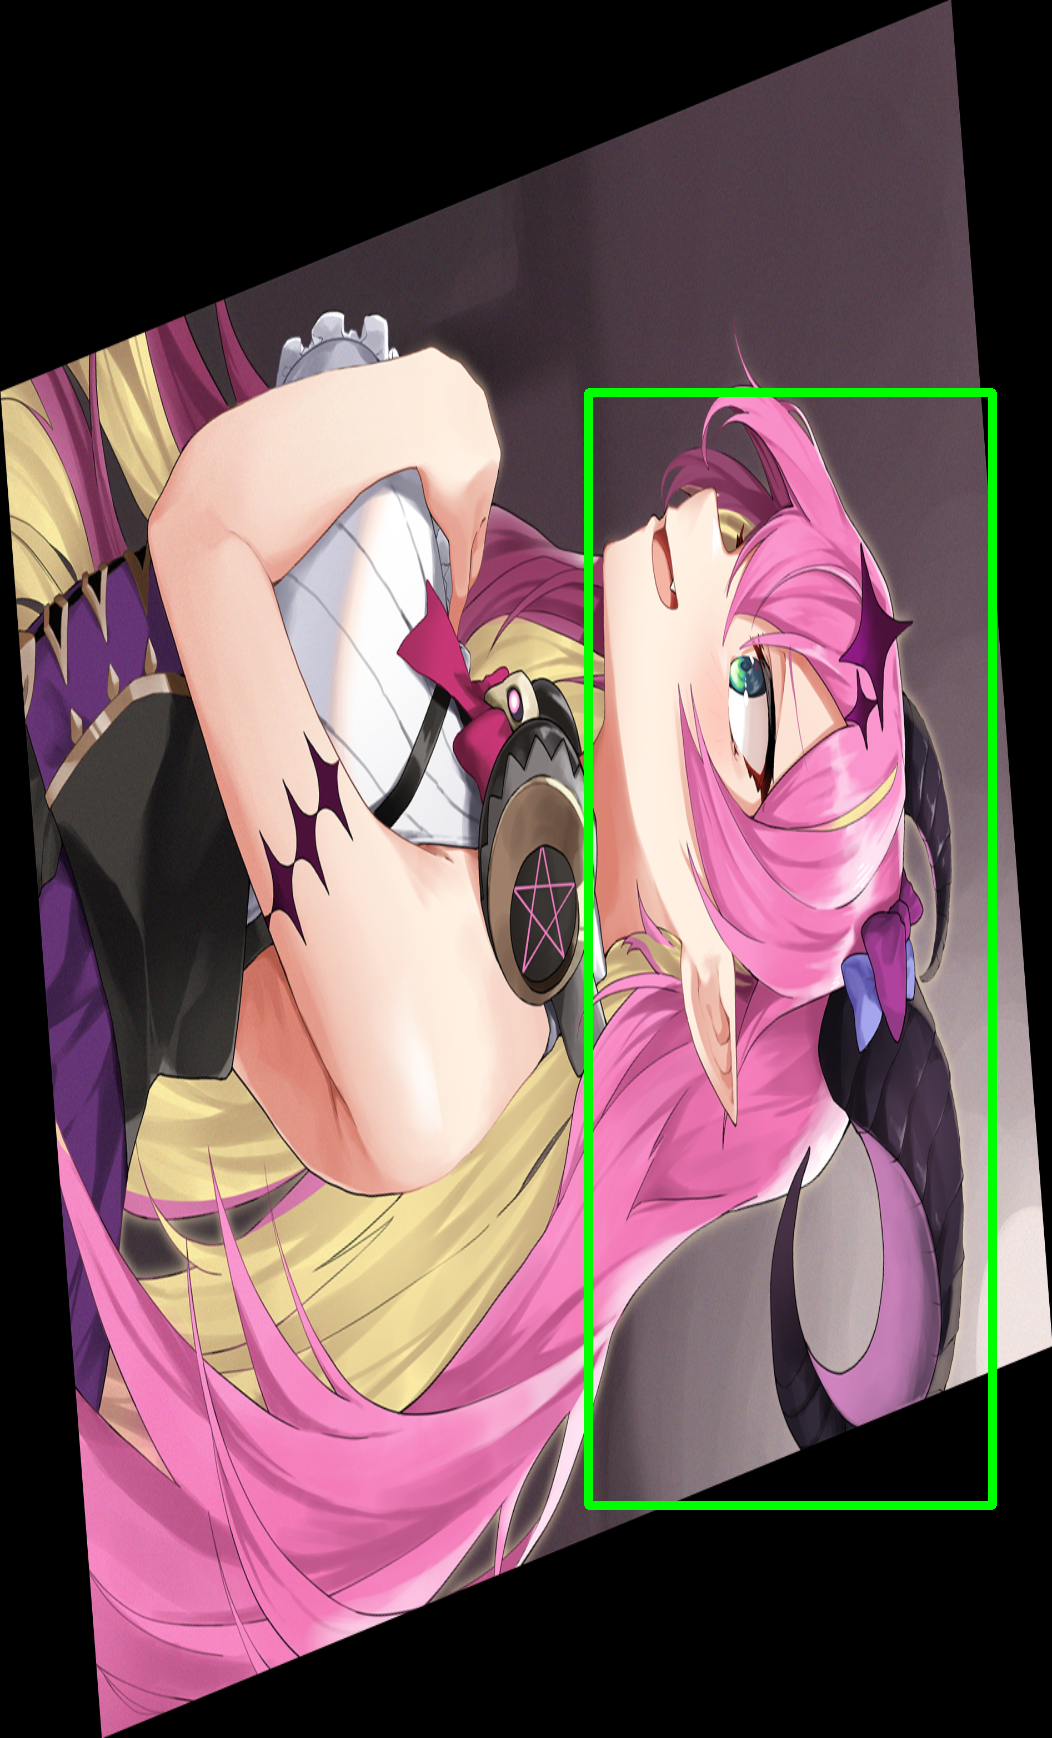
\includegraphics[width=\textwidth]{images/augmentation/Pixiv-83768702_p0-RandomRotate_280-BB.png}
        % \caption{280 degrees}
        \caption{}
        \label{fig:aloe5}
    \end{subfigure}
    \begin{flushleft}
        (a) Original image\cite{83768702}\\
        (b) Rotate with 5 degrees\\
        (c) Rotate with 83 degrees\\
        (d) Rotate with 187 degrees\\
        (e) Rotate with 280 degrees\\
    \end{flushleft}
    \caption{Image Rotation}
    \label{fig:manoaloe1}
\end{figure}